%%%%%%%%%%%%%%%%%%%%%%%%%%%%%%%%%%%%%%%%%%%%%%%%%%%%%%%%%%%%%%%%%%%%%
%
%  This is a sample LaTeX input file for your contribution to
%  the ICTT26 conference.
%
%  Adapted from the ICTT-22 template by T. Palmer (palmerts@ne.orst.edu)
%
%  Please use it as a template for your full paper
%    Accompanying/related file(s) include: class/format file ictt26.cls
%       2. Sample Postscript Figure:   figure.eps
%    Notes:
%      (1) You can use the "dvips" utility to convert .dvi
%          files to PostScript.  Then, use either Acrobat
%          Distiller or "ps2pdf" to convert to PDF format.
%      (2) Different versions of LaTeX have been observed to
%          shift the page down, causing improper margins.
%          If this occurs, adjust the "topmargin" value in the
%          ictt22.cls file to achieve the proper margins.
%
%%%%%%%%%%%%%%%%%%%%%%%%%%%%%%%%%%%%%%%%%%%%%%%%%%%%%%%%%%%%%%%%%%%%%


%%%%%%%%%%%%%%%%%%%%%%%%%%%%%%%%%%%%%%%%%%%%%%%%%%%%%%%%%%%%%%%%%%%%%
\documentclass{ictt26}
%
%  various packages that you may wish to activate for usage
\usepackage{graphicx}
\usepackage{tabls}
\usepackage{afterpage}
\usepackage{lastpage}
%\usepackage{cites}
%\usepackage{epsf}
\usepackage{amsmath, amssymb, bm}
\usepackage{multirow}
\usepackage{tikz}
\usepackage{tikz-3dplot}
\usetikzlibrary{arrows,calc}
\usepackage{subcaption}
%
% Math commands
\newcommand{\mcl}[1]{\ensuremath{\Lambda_{#1}}}
\newcommand{\cl}[1]{\ensuremath{\lambda_{#1}}}
\newcommand{\partialx}[1]{\ensuremath{\frac{\partial {#1}}{\partial x}}}
\newcommand{\derivx}[1]{\ensuremath{\frac{d {#1}}{dx}}}
\newcommand{\aflux}[2]{\ensuremath{\psi\left({#1}, {#2} \right)}}
\newcommand{\cs}[2]{\ensuremath{\sigma_{#1}\left({#2}\right)}}
\newcommand{\src}[1]{\ensuremath{q\left({#1}\right)}}
\newcommand{\csmat}[2]{\ensuremath{\sigma_{#1}^{#2}}}
\newcommand{\scatratmat}[1]{\ensuremath{c_{#1}}}
\newcommand{\sfluxnofn}{\ensuremath{\phi}}
\newcommand{\sfluxmatnofn}[1]{\ensuremath{\sfluxnofn_{#1}}}
\newcommand{\sflux}[1]{\ensuremath{\sfluxnofn \left( {#1} \right)}}
\newcommand{\sfluxmat}[2]{\ensuremath{\sfluxmatnofn{#1}\left( {#2} \right)}}
\newcommand{\sfluxrmserr}[2]{\ensuremath{\sfluxnofn_{#1}^{#2}}}
\newcommand{\ensavg}[1]{\ensuremath{\left<{#1}\right>}}
%
% Shortcut commands
\newcommand{\eq}[1]{Eq.~(\ref{#1})}
\newcommand{\eqnolabel}[1]{(\ref{#1})}
\newcommand{\eqs}[1]{Eqs.~(\ref{#1})}
\newcommand{\eqsthru}[2]{Eqs.~(\ref{#1})--(\ref{#2})}
\newcommand{\eqsand}[2]{Eqs.~(\ref{#1}) and (\ref{#2})}
\newcommand{\tbl}[1]{Table~\ref{#1}}
\newcommand{\tblnolabel}[1]{\ref{#1}}
\newcommand{\tbls}[1]{Tables~\ref{#1}}
\newcommand{\tblsthru}[2]{Tables~\ref{#1}--\ref{#2}}
\newcommand{\tblsand}[2]{Tables~\ref{#1} and \ref{#2}}
\newcommand{\fig}[1]{Fig.~\ref{#1}}
\newcommand{\fignolabel}[1]{\ref{#1}}
\newcommand{\figs}[1]{Figs.~\ref{#1}}
\newcommand{\figsthru}[2]{Figs.~\ref{#1}--\ref{#2}}
\newcommand{\figsand}[2]{Figs.~\ref{#1} and \ref{#2}}
\newcommand{\sxn}[1]{Section~\ref{#1}}
%
%
% Insert authors' names and short version of title in lines below
%
\newcommand{\authorHead}      % Author's names here
   {Daniele Tomatis et Al.}
\newcommand{\shortTitle}      % Short title here
   {The Ronen Method in simple 1-D problems}

\DeclareMathOperator{\sign}{sgn}
\newcommand{\pluseq}{\mathrel{+}=}
%%%%%%%%%%%%%%%%%%%%%%%%%%%%%%%%%%%%%%%%%%%%%%%%%%%%%%%%%%%%%%%%%%%%%
%
%   BEGIN DOCUMENT
%
%%%%%%%%%%%%%%%%%%%%%%%%%%%%%%%%%%%%%%%%%%%%%%%%%%%%%%%%%%%%%%%%%%%%%
\begin{document}

% Fix the large top margin (psb)
\setlength{\topmargin}{-30pt}

%
%      Headers and Footers
\afterpage{%
\fancyhf{}%
\fancyhead[CE]{
{\scriptsize \authorHead}}
\fancyhead[CO]{
{\scriptsize \shortTitle}}
%\lfoot{\scriptsize{%
%26th International Conference on Transport Theory (ICTT-26) \\
%Sorbonne University, Paris, France, 2019}}%
%\rfoot{\thepage/\totalpages{}}%
\rfoot{\thepage/\pageref{LastPage}}%
\pagestyle{fancy}
}

\normalsize

\setlength{\baselineskip}{16.8pt}
\vspace{-3pt}

%
% TITLE
%

\begin{center}
\textbf{\large \\%
%NEUTRON DIFFUSION BY THE RONEN METHOD IN HETEROGENEOUS MEDIA
ON THE RONEN METHOD IN SIMPLE 1-D PROBLEMS
}

%
% FIRST AUTHORS
%
\setlength{\baselineskip}{12pt}
\textbf{Daniele Tomatis}\\
DEN, Service d'{\'e}tudes des r\'eacteurs et de math\'ematiques appliqu\'ees (SERMA),\\
CEA, Universit\'e Paris-Saclay, F-91191 Gif-sur-Yvette, France\\
daniele.tomatis@cea.fr\\
\vspace{0.25in}
\textbf{Roy Gross and Erez Gilad}\\
The Unit of Nuclear Engineering\\
Ben-Gurion University of the Negev, Israel\\
roygros@post.bgu.ac.il, gilade@bgu.ac.il\\
\end{center}

\begin{abstract}
In this work we apply the Ronen method to resolve the neutron transport in simple homogeneous problems. Slab, cylindrical and spherical geometries are studied. This method demands successive resolutions of the diffusion equation, where the local diffusion constants are modified in order to reproduce new estimates of the currents by a transport operator. The diffusion solver employs here finite differences and the transport-corrected currents are forced in the numerical scheme by means of drift terms, like in the CMFD scheme. Boundary conditions are discussed introducing proper approximations to save the particle balance in case of reflection in the slab. The solution from the Ronen iterations is compared against reference results provided by the collision probability method (CPM). More accurate estimates of the currents are provided by integral equations using first flight escape probabilities. Slow convergence on the scalar flux is analyzed, although the results match the reference solutions in the limit of fine meshes and far from the bare boundary.
%
%In this work we apply the Ronen method in the slab geometry filled with heterogeneous media. Neutron diffusion is solved by a nodal method on a coarse mesh, while reference solutions of the neutron distribution are provided by a discrete ordinate transport solver. The CMFD technique is used for both the implementation of the nodal solver and for the corrections of the diffusion coefficient given by the Ronen method. The presence of discontinuity factors for equivalencing the diffusion solution is investigated jointly with the Ronen method. Results are presented for different levels of material heterogeneity at the slab interfaces.
\end{abstract}
%
\clearpage
\tableofcontents
\clearpage
%
% SET RAGGED RIGHT MARGIN
%
\raggedright

\section{INTRODUCTION}
\label{sec:intro}

In 2004 Ronen suggested to calculate more accurate currents by means of an integral transport operator still using a neutron flux computed in diffusion theory \cite{ronen2004accurate}. This allowed having new estimates of the diffusion coefficient still using Fick's law. Since these estimates need a known flux distribution, it was also suggested to execute new diffusion calculations, thus updating iteratively the diffusion coefficient in the global calculation. The main reason motivating this method was to overcome the underlying limitation of Fick's law requiring low flux gradients, and so low neutron absorption and high scattering in general. Nevertheless, isotropic scattering remained as a basic postulate.

This idea was later used by Tomatis and Dall'Osso, who provided a numerical demonstration in a simple slab problem \cite{tomatis2011application}. Instead of updating the diffusion coefficient by the ratio of the current exchange and the flux gradient, as in Fick's law, they recurred to the scheme of the coarse mesh finite differences method (CMFD) for taking into account the new currents estimated by the integral transport operator in the diffusion solver.
%
%They proposed to update non-linearly the diffusion coefficients at the cell interfaces of the spatial mesh by the coarse mesh finite differences method (CMFD).
%
This technique, largely adopted in the literature of nodal methods \cite{smith1983nodal,lawrence1986progress}, can avoid indeterminate divisions in case of vanishing current and flux gradient. They tested this implementation in a bare slab with two-group cross sections homogenized in a realistic PWR assembly. It was observed that the Ronen method (RM) could drive the flux from diffusion towards the reference of the integral Boltzmann transport equation, regardless of the initial formulation used for the diffusion coefficient. Remarkably, the unphysical zero-flux boundary condition was not preventing to correct the flux near the boundary, that is within a few mean free paths. However, higher errors were noticed at the boundary with vacuum, slowly decreasing even after many iterations.% Their work was limited to the homogeneous slab, and resolved neutron diffusion on the same discretized spatial mesh used for the reference from neutron transport.
%
%In this work, we study the Ronen method with coarse meshes in order to approach the typical situation of core calculations, where homogenized cross sections are prepared in single fuel assemblies by lattice transport calculations. Nodal expansion methods are generally used with coarse meshes relying on polynomial-like or semi-analytical solutions \cite{lawrence1986progress}. They can also employ the discontinuity factors in their solving equations, thus yielding an equivalent form to the reference transport solution \cite{smith1986assembly}. Its implementation through the CMFD compensates the truncation errors caused by the approximate finite differences, and eases the global resolution to many local two-nodes problems. Of course, the simplified 1-D geometry let us disregard here all issues related to the transverse leakage approximation.
%
%Specifically, we compare hereafter the solutions obtained by the Ronen method and by the analytical nodal method, with the aim to present the first method as an on-line equivalence technique, farther capable to fulfill the neutron transport in its integral form on the coarse mesh. %We also use the discontinuity factors to enforce the physical equivalence between diffusion and transport, which is not preserved after the common flux-volume weighting homogenization of the cross sections. The implementation of both methods uses the CMFD, as shown in section \ref{sec:impl}. The basics of the analytical nodal method are reported in section \ref{sec:nd}, while the procedure to estimate the currents by the integral transport operator follows in section \ref{sec:ce}. New transport-corrected boundary conditions are derived in section \ref{sec:bc} to fix the bad performances observed in \cite{tomatis2011application}. The results on a few characteristic configurations are discussed in section \ref{sec:res}. Finally, the article ends with the conclusion in section \ref{sec:cncls}.

In this work we investigate further the convergence on the first flux moments, aiming to extend the study to the cylindrical and spherical geometries with homogeneous media. The details of the implementation of the Ronen method in the diffusion solver are presented in section \ref{sec:impl}, while the procedure to estimate the currents by the integral transport operator follows in section \ref{sec:ce}. Boundary conditions are derived in section \ref{sec:bc}. The results on a few characteristic configurations are discussed in section \ref{sec:res}. Finally, the article ends with the conclusion in section \ref{sec:cncls}.


\section{IMPLEMENTATION}
\label{sec:impl}

The cross sections, as well as the diffusion coefficient, are usually available as volume-averaged data per cell in the mesh. A lattice transport computer code can prepare these data by homogenization. Once the scalar flux is known from the finite differences solver using the original diffusion coefficients, the integral expressions derived in section \ref{sec:ce} can be used to get new estimates of the current $J$ at the cell interfaces. %Alternatively, new current estimates can come from the two-nodes problem resolved by the nodal method in section \ref{sec:nd}.
Instead of computing new diffusion coefficients on the same interfaces straight by Fick's law, $J = -D \partial_x \phi$, we obtain new corrective currents $\delta J = J - \Upsilon$ that are supplied next to the neutron balance in diffusion. Here $\Upsilon$ is the current obtained with the original values of the diffusion coefficient and with the derivative approximated by finite differences. In 1-D %Cartesian
geometry and using the notation in Fig. \ref{fig:mesh1D}, it is:
\begin{equation}
  \Upsilon_{i+1/2} = -2 D_{i+1/2} \frac{\phi_{i+1} - \phi_{i}}{\Delta_{i+1} + \Delta_{i}}, \text{ for } i = 0, \ldots, I-1,
  % \Upsilon^{(i+1/2)} = -2 D^{(i+1/2)} \frac{\phi_{i+1} - \phi_{i}}{\Delta_{i+1} + \Delta_{i}}, \text{ for } i = 0, \ldots, I-1,
  % \Upsilon^{(i+1/2)} = -2 D^{(i+1/2)} \frac{\phi_{i+1} - \phi_{i}}{V_{i+1} + V_{i}}, \text{ for } i = 0, \ldots, I-1,
  \label{eq:cmfd}
\end{equation}
where $\Delta_i = (x_{i+1/2} - x_{i-1/2})$. Integer and rational subscripts indicate cell-averaged and interface quantities, respectively.
%
\begin{figure}[b]
\centering
\input{figures/mesh1d.tkz}
\caption{Notation of the 1-D mesh.}
\label{fig:mesh1D}
\end{figure}
Since the input diffusion coefficients are provided as volume-averaged, and that they are always needed at interfaces, we approximate them by local volume averages:
\begin{equation}
  % D^{(i+1/2)} = \frac{D_{i+1}c_{i+1}\Delta_{i+1} + D_{i}c_i\Delta_{i}}{c_{i+1}\Delta_{i+1} + c_i\Delta_{i}}, \text{ for } i = 0, \ldots, I-1.
  % D^{(i+1/2)} = \frac{D_{i+1} V_{i+1} + D_{i} V_i}{V_{i+1} + V_i}, \text{ for } i = 0, \ldots, I-1.
  D_{i+1/2} = \frac{D_{i+1} V_{i+1} + D_{i} V_i}{V_{i+1} + V_i}, \text{ for } i = 0, \ldots, I-1.
  \label{eq:dc0}
\end{equation}
The values of the diffusion coefficient at $-1/2$ and $I-1/2$ are simply the coefficients of the boundary cells. $V_i$ is the reduced volume in the $i$-th cell, that is determined along the only dimension of interest. It is then per unit of transverse surface in the slab, the unit azimuthal angle in the cylinder and per unit cone in the sphere. Specifically, $V_i = \Delta_i c_i$ with $c_i$ depending on the system of coordinates. The $c$ coefficients are unitary in the Cartesian frame. In the cylinder, $c_i = x_i$ for all $i$ with $x_i = (x_{i-1/2} + x_{i+1/2}) / 2$ (arithmetic mean), whereas $c_i = (4 x_i^2 - \hat{x}_i^2)$ in the sphere with $\hat{x}_i = \sqrt{x_{i-1/2} x_{i+1/2}}$ (geometric mean).
%
The discretized form of the current $\delta J$ must involve the flux in order to be taken into account in the finite differences equations. Its representation is changed into a drift-advection term determined by the neighboring cell fluxes, thus avoiding possible undefined division by zeros in case of flat flux \cite{smith1983nodal}:
\begin{equation}
  \delta J_{i+1/2} = -2 \delta D_{i+1/2} \frac{\phi_{i+1} + \phi_{i}}{\Delta_{i+1} + \Delta_{i}}, \text{ for } i = 0, \ldots, I-1.
  % \delta J^{(i+1/2)} = -2 \delta D^{(i+1/2)} \frac{\phi_{i+1} + \phi_{i}}{\Delta_{i+1} + \Delta_{i}}, \text{ for } i = 0, \ldots, I-1.
  % \delta J^{(i+1/2)} = -2 \delta D^{(i+1/2)} \frac{\phi_{i+1} + \phi_{i}}{V_{i+1} + V_{i}}, \text{ for } i = 0, \ldots, I-1.
  \label{eq:dj}
\end{equation}
This allows determining the new numerical corrections $\delta D$ to use in the finite differences solver, together with the diffusive currents from \eq{eq:cmfd}. If necessary, the spatial differences at the denominator of Eq. \ref{eq:dj} can be removed by reason of the arbitrary definition used for $\delta D$. Finally, the neutron balance resolved by the CMFD takes into account both types of currents $\Upsilon$ and $\delta J$. Non-linear iterations with new corrections given by $\delta J$ are needed because of their dependence on the unknown flux.

The divergence operator used in the multi-group balance equation can be described with the general form $d_x (x^b J_g)/ x^b$, with $b = 0$, $1$ and $2$ respectively for the slab, for the cylinder and for the sphere. We solve then for the volume-integrated flux,
\begin{equation*}
  \hat{\phi}_{g,i} = \int_{x_{i-1/2}}^{x_{i+1/2}}{ x^b \phi_g(x) dx } = \bar{\phi}_{g,i} V_i,
\end{equation*}
making the approximation that the average group flux $\bar{\phi}_{g,i} \approx \phi_{g,i}$ in the equations above.


\section{CURRENT ESTIMATION}
\label{sec:ce}

\subsection{Slab geometry}
\label{sec:slab}
The angular flux from the integral transport equation (with standard notation) is:
\begin{equation}
\varphi(x, \mu) = \varphi(x_b, \mu) e^{-\tau(x_b, x)/\mu} + \int_{x_0}^x {dx' \frac{q(x', \mu)}{\mu} e^{-\tau(x', x)/\mu}},
\label{eq:NTE}
\end{equation}
with the optical length $\tau(x_1, x_2) = \int_{x_1}^{x_2}{dx' \sigma_t(x')}$. Contrary to other formulations, we do not include the direction cosine of the neutron velocity $\mu$ in the definition of the optical length to ease the numerical integrations in the following. Eq. \ref{eq:NTE} holds for both positive directions $(\mu > 0)$ where $x_0 = x_{-1/2} = a$, and negative ones $(\mu > 0)$ where $x_0 = x_{I-1/2} = b$. The inclusion of the energy variable in Eq. \ref{eq:NTE} is straightforward; we use hereafter the multi-group theory, writing the source $q_g$ as\footnote{Curly brackets remind the possible use of the $k$-eigenvalue in case of vanishing external sources.}:
\begin{equation}
\label{eq:srcg}
q_g = \sum_{g'=1}^G{\left[
  \sum_{l=0}^\infty{ \frac{2l+1}{2}\sigma_{s,l, g' \rightarrow g}(x)P_l(\mu)\varphi_{l,g'}(x)
  + \frac{\chi_g}{2\{k\}} \nu\sigma_{f,g'}(x)\phi_{g'}(x)}\right] + S_g
                 },
\end{equation}
where the subscript $l$ refers to the moments of the expansions of the flux and of the scattering cross section on the Legendre polynomials $P_l$. Fission emission is isotropic, so that only the scalar flux $\phi$ being equal to the first moment $\varphi_0$ is retained for the fission term. Without the external source $S$, the multiplication factor $k$ is used as eigenvalue to avoid the only trivial vanishing solution. Since $q$ is computed by the results of the diffusion equation in the Ronen method, $l$ can only assume the values 0 and 1, with the second moment $\varphi_1$ equal to the net current $J$.% Hereafter we consider only isotropic sources.

Multiplication of Eq. \ref{eq:NTE} by $\mu$ and the integration over $[-1, 1]$ provides the expression for the current, see \cite{tomatis2011application}. The integration on $\mu$ yields integral exponential functions by a simple change of variable ($\mu = \pm 1/u$, according to the sign of $\mu$) \cite{AS1964handbook}:
\begin{equation*}
E_n(\tau) = \int_0^1{d\mu\, e^{-\tau / \mu} \mu^{n-2}} = \int_1^\infty{du\, e^{-\tau u}u^{-n}}, \: n \geq 0.
\end{equation*}
These special functions are then used to compute the current at the cell interfaces for all $i$:
\begin{equation}
\begin{split}
% J_g(x_{i+1/2}) &=
J_{g,i+1/2} &= \int_0^{ 1}{d\mu\, \mu \varphi_g(a, \mu) e^{-\tau_g(a, x_{i+1/2})/\mu}}
             - \int_0^{-1}{d\mu\, \mu \varphi_g(b, \mu) e^{-\tau_g(b, x_{i+1/2})/\mu}}\\
  & + \sum_{j=0}^{I-1} \left[  \sign(x_{i+1/2} - x_{j+1/2}) \frac{q_{0,g,j}}{2} \int_{x_{j-1/2}}^{x_{j+1/2}}{dx' E_{2}\left(\lvert \tau_g(x', x_{i+1/2}) \rvert \right) } \right.\\
  & \left. \qquad+ \frac{3}{2}q_{1,g,j} \int_{x_{j-1/2}}^{x_{j+1/2}}{dx' E_{3}\left(\lvert \tau_g(x', x_{i+1/2}) \rvert \right) }\right],
\end{split}
\label{eq:J_tr}
\end{equation}
where $q_{(.),g,j}$ are the moments of the souce $q_g$ from Eq. \ref{eq:srcg} averaged in the volume of the $j$-th cell:
\begin{subequations}
\label{eq:srclg}
\begin{align}
   q_{0,g,j} &= \sum_{g'}\left(\sigma_{s,0,g' \rightarrow g,j} +
                              \chi_g \nu\sigma_{f,g',j}
                        \right) \phi_{g',j},\label{eq:srclg0}\\
   q_{1,g,j} &= \sum_{g'}\sigma_{s,1,g' \rightarrow g,j}J_{g',j}.\label{eq:srclg1}
\end{align}
\end{subequations}
The current appearing in $q_{1,g,j}$, that is in case of linearly anisotropic scattering, is also to be considered as volume-averaged in the cell $j$. The optical lengths show the subscript $g$ because they are evaluated with the corresponding total cross section $\sigma_{t,g}$. For the property $E'_{n+1}(\ell) = -E_n(\ell)$, the spatial integrals of the integral exponential functions can be solved analytically by integrating on $\tau$:
\begin{equation*}
\begin{aligned}
\int_{x_{j-1/2}}^{x_{j+1/2}}{ dx' E_{n}\left(\lvert \tau_g(x', x_{i+1/2}) \rvert \right) } =
\frac{\sign(x_{i+1/2} - x_{j+1/2})}{\sigma_{t,g,j}} \cdot \\
\left[
  E_{n+1} \left(\lvert \tau_g(x_{j+1/2}, x_{i+1/2}) \rvert \right)
 -E_{n+1} \left(\lvert \tau_g(x_{j-1/2}, x_{i+1/2}) \rvert \right)
\right].
\end{aligned}
\end{equation*}
These quantities can be computed for $i > j$ only, because the others are simply opposite in sign (anti-symmetric). Eq. \ref{eq:J_tr} can be reformulated for the partial currents, thus considering only the contributions coming from the different sides of $x_{i+1/2}$. Omitting the index on groups and keeping only isotropic sources, this is:
\begin{equation}
\label{eq:pcslab}
  J^\pm_{i+1/2} = \sum_{j=1}^I{q_{0,j} \Delta_i \tilde{e}^\pm_{i+1/2,j} + J^\pm(x_b) \tilde{t}_{i+1/2, x_b}}.
\end{equation}
$\tilde{e}_{i+1/2, j}$ represents the probability of a neutron emitted isotropically in $\Delta_i$ to escape uncollided at $x_{i+1/2}$, along its positive or negative direction of flight. $\tilde{t}_{i+1/2, x_b}$ is the transmission probability of a neutron to enter isotropically at $x_b$ and to cross the interface at $x_{i+1/2}$ without colliding hitherto.


\subsection{Cylindrical geometry}
\label{sec:cylinder}

The expression of the current in curvilinear geometries is derived in this section from the 3-D Cartesian geometry, where the angular flux at the point $\mathbf{r}$ along the direction of flight $\mathbf{\Omega}$ is given by the general expression \cite{lewis1984computational}:
\begin{equation}
\varphi(\mathbf{r}, \mathbf{\Omega}) = \int_0^{S'}{ds'\, q(\mathbf{r} - s' \mathbf{\Omega}, \mathbf{\Omega}) \exp(-\tau(\mathbf{r}, \mathbf{r} - s' \mathbf{\Omega}))} + \varphi(\mathbf{r} - S' \mathbf{\Omega}, \mathbf{\Omega}) \exp(-\tau(\mathbf{r}, \mathbf{r} - S' \mathbf{\Omega})),
\label{eq:ITE_angflx}
\end{equation}
that is considering the contribution of the source $q$ within the distance $S'(\mathbf{r}, \mathbf{\Omega})$ from the boundary and the possible entering amount of particles therein. All contributions are collected at $\mathbf{r}$ by exponential attenuation along the travelled optical path, that is according to the probability of still continuing the first flight after emission. We examine first the case of the cylinder as a particular case of the 2-D frame. In planar geometry the angular flux and the source do not depend on the axial coordinate $z$. Hence, the position on the characteristic line identified by $\mathbf{\Omega}$ is projected on the $x$-$y$ plane (see Fig. \ref{fig:fullframe}): $\varphi(\mathbf{r} - s' \mathbf{\Omega},\mathbf{\Omega}) =\allowbreak \varphi(\mathbf{r} - s \mathbf{\Omega}_p,\mathbf{\Omega})$ and likewise for $q$, with the unit vector $\mathbf{\Omega}_p$ lying on the $x$-$y$ plane. $\theta$ is the polar angle measured between $\hat{e}_z$ and $\mathbf{\Omega}$. In absence of incoming particles, this allows to rewrite Eq. \ref{eq:ITE_angflx} as:
\begin{equation}
\varphi(\mathbf{r}, \mathbf{\Omega}) = \int_0^S{ds\, \frac{q(\mathbf{r} - s \mathbf{\Omega}_p, \mathbf{\Omega})}{\sin \theta} \exp \left[ -\frac{\tau(\mathbf{r}, \mathbf{r} - s \mathbf{\Omega}_p)}{\sin \theta} \right]}. % + \varphi(\mathbf{r} - S \mathbf{\Omega}_p, \mathbf{\Omega}) \exp(-\frac{\tau(\mathbf{r}, \mathbf{r} - S' \mathbf{\Omega})}{\sin \theta}).
\label{eq:ITE_xy}
\end{equation}

As well, integration of Eq. \ref{eq:ITE_xy} over the solid angle $d\mathbf{\Omega} = \sin \theta d\omega d \theta$ yields the scalar flux at the point $\mathbf{r}$. The theory of collision probability methods originates from the use of flat isotropic sources in the cells of the spatial mesh. The use of anisotropic sources with spatial variation in the same cells, for instance polynomial-like, is possible but leads to much more difficult expressions to solve. Two integrations in space arise for each direction $\mathbf{\Omega}$, connecting the source in region $j$ to the flux (or its total reaction rate) in region $i$ by means of its collision probability. The incoming flux is usually considered as isotropic too, or linearly anisotropic in angle as in \cite{hebert2009applied} to relate the partial entering and outgoing currents to the only first flux moments. These partial currents on the boundary must satisfy a general condition of albedo.

Using standard nomenclature of collision probability methods, transfer probabilities refer to particles entering the problem domain and leaving it without incurring into any collision. They can provide the probability of reflection in case the entering and the leaving surfaces are the same. The probability of escape deals with neutrons produced in a given region and leaving a surface, still uncollided. These probabilities are employed to write the integral transport equations for the volume-averaged scalar flux (or its total reaction rate) in each cell, and the surface-averaged currents at the cell interfaces.

The projections of partial currents on the outward normal $\hat{n}$ to a given surface are obtained from integration of Eq. \ref{eq:ITE_xy} in $d\mathbf{\Omega}$ with the weight $| \hat{n} \cdot \mathbf{\Omega} | = \sin \theta | \hat{n} \cdot \mathbf{\Omega}_p |$ on $\hat{n} \cdot \mathbf{\Omega} \lessgtr 0$. Higher moments can be obtained by the weights associated to the corresponding spherical harmonics. Integration along the polar angle is resolved analytically by the Bickley-Naylor functions \cite{amos1983uniform}:
\begin{equation}
\text{Ki}_n(\tau) = \int_0^{\pi/2}{ d\theta \sin^{n-1} \theta \exp\left(-\frac{\tau}{\sin \theta}\right) },\: n \geq 0.
\label{eq:Kin}
\end{equation}
The properties used for the computation of these functions are available elsewhere \cite{lewis1984computational,hebert2009applied}. We use the fortran library by Amos from 1983 in this work \cite{amos1983algorithm}.

\begin{subequations}
After introducing these arguments for a bare cylinder, the current leaving the cylindrical surface at $\mathbf{r}$ (with direction $\hat{n}$) given by neutrons flying along $\mathbf{\Omega}_p$ is:
\begin{equation}
J^+(\mathbf{r}) = \frac{1}{2\pi}\int_{W^+}{
  d\omega\, | \hat{n} \cdot \mathbf{\Omega}_p | \,
  \int_0^S ds\, \text{Ki}_2\left[ \tau\left(\mathbf{r}, \mathbf{r} - s \mathbf{\Omega}_p \right)\right]
  q(\mathbf{r} - s \mathbf{\Omega}_p)},
\label{eq:currp_cylinder1}
\end{equation}
with $W^+ = \left\{\omega \mid \hat{n}\cdot \mathbf{\Omega}_p > 0\right\}$. Using the surface element $dA' = s d\omega ds$ and $\mathbf{r}'_p = \mathbf{r} - s \mathbf{\Omega}_p$, it is also:
\begin{equation}
J^+(\mathbf{r}) = \int_{W^+ \times [0, S]}{
  dA'\, \hat{n} \cdot (\mathbf{r} - \mathbf{r}'_p) \,
  \frac{\text{Ki}_2\left[ \tau\left(\mathbf{r}, \mathbf{r}'_p \right)\right]}{2 \pi \lvert \mathbf{r} - \mathbf{r}'_p \rvert^2}
  q(\mathbf{r}'_p)}.
\label{eq:currp_cylinder2}
\end{equation}
\label{eq:currp_cylinder}
\end{subequations}
$J^-$ is obtained with integration over $w \in W^- =  \left\{\omega \mid \hat{n}\cdot \mathbf{\Omega}_p < 0\right\}$ instead.% The coefficient $1/2\pi$ comes from the probability of isotropic angular redistribution applied to the source $q$.

Another integration on the total surface $S(r) = \int{r d\theta'} = 2\pi r$, with $\theta' = \hat{n}\cdot \mathbf{\Omega}_p$, is necessary to obtain the current density in the 1-D frame. For a given angle $\omega$, we have then volume integrals to solve numerically along many parallel lines called tracks, see Fig. \ref{fig:cyltracks}, for $r d\theta' = dh/\cos \theta'$. Furthermore, the tracks are identical for any angle $\omega$ in the 1-D cylindrical geometry factoring out $2\pi$ from the integrals in Eqs. \ref{eq:currp_cylinder}, which can also be limited to half portion of the cylinder thanks to its symmetry. Finally, the outgoing and incoming currents at $r$ become:
\begin{equation}
% J^\pm(r) = \pm \frac{1}{\pi r^2} \int_0^r { dh\, y
J^\pm(r) = \pm \frac{1}{\pi r} \int_0^r { dh\,
    \int_{-Y}^{\pm y}{d \ell \,
      \text{Ki}_2\left[\tau( y, y - \ell )\right] q(h, y - \ell)}}
\label{eq:currp_cyl_atr}
\end{equation}
with $y(r,h) =\sqrt{r^2 - h^2}$, $Y = y(R,h)$ and the outer radius $R$. After multiplication by $S(r)$ and still with uniform sources, Eq. \ref{eq:currp_cyl_atr} can be written in terms of the escape probability $\tilde{e}_{j}(r)$ for a neutron to be emitted isotropically in ring $j$ and to leave uncollided along the normal direction the semicylinder surface at $r$, being crossed with angle $\omega \in W^\pm$:
\begin{equation}
J^\pm(r)S(r) = \sum_j q_j V_j \left[ \pm \tilde{e}^\pm_j(r) \right] \mbox{ with }
% e^\pm_j(r) = \frac{2}{r V_j} \int_0^r { dh\, y
\tilde{e}^\pm_j(r) = \frac{2}{V_j} \int_0^r { dh\,
  \int_{L^\pm_j}{d \ell \, \text{Ki}_2\left[\tau( y, y - \ell )\right]}},
\label{eq:esc_prob_cyl}
\end{equation}
$L^\pm_j(h) = [-Y,\pm y] \cap V_j$ and where $V_j$ is the ring area. $\text{Ki}_2\left[\tau( y, y - \ell )\right]$ is the transport kernel expressing the probability of a neutron to travel uncollided along $\omega$ for a lenght $\tau$, given in mean free path units, from $(y - \ell)$ to $y$ \cite{stamm1983methods}. The integral on the track $\ell$ is written differently for the convex and for the concave parts of the rings with respect to the direction of flight, see for instance track 1 and 2 in Fig. \ref{fig:cyltracks} where the same notation of Fig. \ref{fig:mesh1D} is used for the radial mesh. The current leaving the $i$-th ring at $r_{i+1/2}$ gets all source contributions weighted with the quantities $\varepsilon^+_{i+1/2,j} = V_j \tilde{e}^+_{i+1/2,j}$:
%
\newlength{\plussign}
\settowidth{\plussign}{$+$}
%
\begin{equation}
\label{eq:esc_prob_cyij}
  \begin{gathered}
  % \varepsilon^+_{i+1/2,j} = \frac{2}{r_{i+1/2}} \cdot\\
  \varepsilon^+_{i+1/2,j} = 2\: \cdot\\
  %\left\{
  \begin{cases}
%  \displaystyle ~\int_0^{r_{i-1/2}} { dh\, y
  \displaystyle ~\int_0^{r_{i-1/2}} { dh\,
    \int_0^{\ell_j}{ d\ell \bigg[ }}\\[3mm] \qquad
      \displaystyle \hspace{\the\plussign}
        \text{Ki}_2\left(2 \sigma_i \ell_i + \tau_{ii} + \tau_{ij} + \sigma_j \ell \right)
        \text{ if } i < j \\[3mm] \qquad
      \displaystyle +
        \text{Ki}_2\left(\sigma_i \ell_i + (1 - \delta_{ij})(\tau_{ij} + \sigma_j \ell_j) + \tau_{jj} + \sigma_j \ell \right)
        \text{ if } i \geq j \\[3mm] \qquad
      \displaystyle +
        \text{Ki}_2\left((1 - \delta_{ij})(\sigma_i \ell_i + \tau_{ij}) + \sigma_j \ell \right)
        \text{ if } i \geq j \\
%
%  \displaystyle + \int_0^{r_{i-1/2}} { dh\, y
%    \int_0^{\ell_j}{ d\ell \, \left[
%      \text{Ki}_2\left(\sigma_i \ell_i + \tau_{ij} + \sigma_j \ell_j + \tau_{jj} + \sigma_j \ell \right)
%      \right. }} \\ {{ \left.
%      + \text{Ki}_2\left(\sigma_i \ell_i + \tau_{ij} + \sigma_j \ell \right) \right]} }
%  \text{ if } i \geq j\\
%
  \displaystyle \: \bigg] +\int_{r_{i-1/2}}^{r_{i+1/2}} { dh\, y
    \int_0^{\ell_j}{ d\ell \, \text{Ki}_2\left((1-\delta_{ij})(\sigma_i \ell_i + \tau_{ij}) + \sigma_j \ell \right)} }
  \text{ if } i \leq j,\\
  \end{cases}
  %\right.
  \end{gathered}
\end{equation}
using the Kronecker function $\delta_{ij} = 1$ only if $i=j$ and null otherwise. $\tau_{ij}$ and $\tau_{ii}$ are respectively the optical lengths between the rings $i$ and $j$, and across the outer diameter of ring $i$. The radial integral includes all rings within $r_{i+1/2}$. The integrals involving the Ki function are solved thanks to the property $d_{\tau}\text{Ki}_n(\tau) = -\text{Ki}_{n-1}(\tau)$.

The corresponding form for the reduced escape probability for the incoming current is:
\begin{equation}
\label{eq:esc_prob_cyij-}
%  \varepsilon^-_{i+1/2,j} = \frac{2}{r_{i+1/2}}
  \varepsilon^-_{i+1/2,j} = 2
    \displaystyle ~\int_0^{r_{i+1/2}} { dh\, % y
        \int_0^{\ell_j}{
            d\ell \text{Ki}_2 \left(\tau_{ji} + \sigma_j \ell \right)
        }
	},
\end{equation}
for $i<j$, whereas $\varepsilon^-_{i+1/2,j}\equiv 0$ for $i\geq j$ since in this case a neutron born in volume $j$ (or in volume $j=i$) cannot enter volume $i$ through its outer surface at radius $r_{i+1/2}$ without undergoing a collision. The useful reciprocity and conservation properties commonly used in CPM solvers to save the total computational effort can be applied only after calculating the first flight collision probabilities.

Singularity of the integrand for the $h$-integration is known in the convex part while computing the collision probabilities \cite{hebert2009applied,stamm1983methods}; this notably happens at the outer radius of the $j$-th ring where $\hat{n}$ is perpendicular to $\mathbf{\Omega}_p$. However, that integral can be regularized by a suitable change of variable, see appendix \ref{sec:apx_Flurig}. The calculation of the escape probabilities as presented in this section is %not affected by this problem because of the factor $y$ that comes from the cosine of the angle described by the normal $\hat{n}$ and $\mathbf{\Omega}_p$, which cancels the endpoint singularity.
also affected by this endpoint singularity. Because of this singularity, the integral in $h$ can then be resolved numerically with weights and points by the Gauss-Jacobi quadrature, which is one order more accurate than the common Gauss-Legendre quadrature.

\begin{figure}[htbp]
  \centering
  \begin{minipage}[c]{.5\textwidth}
    \centering
    {%
    \input{figures/fullframe.tkz}
    \caption{Projection of vectors on the $x$-$y$ plane.}
    \label{fig:fullframe}
    }%
    \vspace{3mm}
    \vfill
    {%
    \input{figures/sphere.tkz}
    \caption{Use of symmetry in the sphere for integration over the surface.}
    \label{fig:sphere_tracks}
    }%
\end{minipage}%
\begin{minipage}{.5\textwidth}
  \centering
    \input{figures/cyltracks.tkz}
    \caption{Integration along the tracks in the 1-D cylindrical geometry (suggested by Fig. 3.17 of reference \cite{hebert2009applied}).}
    \label{fig:cyltracks}
\end{minipage}%
\end{figure}

\subsection{Spherical geometry}
\label{sec:sphere}

The derivation of the scalar flux and of the current in the sphere follows the same rational adopted in section \ref{sec:cylinder} by angular integration of Eq. \ref{eq:ITE_angflx} and exploiting the symmetries available in the given coordinate frame. Because of the rotational symmetry any direction of flight lays on a spherical cut passing through the origin ($\mathbf{\Omega}_p = \mathbf{\Omega}$), see Fig. \ref{fig:sphere_tracks}. The integration to carry for each direction $\mathbf{\Omega}$ over the spherical surface $S(r) = \int{r^2\sin \theta' d\theta' d\omega'} = 4\pi r^2$ shows a case similar to the cylinder of Fig. \ref{fig:cyltracks}, with integration on the semi-circle along the coordinate $h$, thanks to the axial symmetry around $\omega'$ that factors out $2\pi$, but with the new weight $h = r\sin \theta'$. The tracking integrals up to the spherical surface are the same for all directions, so that the integration over the unit solid angle yields simply $4\pi$, cancelling out the probability of isotropic emission used for the source. Fig. \ref{fig:sphere_tracks} is specific to the calculation of the positive radial partial currents. Negative partial currents need to consider the sources outside the depicted sphere of integration.

%Thanks to the central symmetry tracking integrals are the same for all directions, so that integration is carried on a semi-circle only, as in the case of the cylinder in Fig. \ref{fig:cyltracks}. Still by referring to Fig. \ref{fig:cyltracks}, we note that $\sin \theta = h/r$ and $\cos \theta = y/r$ with $y$ defined in Eq. \ref{eq:currp_cyl_atr}.
Using the same quantities defined in Eq. \ref{eq:currp_cyl_atr}, Eq. \ref{eq:esc_prob_cyl} holds also for the sphere but using the new reduced escape probability:
\begin{equation}
% \varepsilon_j(r) = \frac{2\pi}{r} \int_0^r { dh\, y
\varepsilon_j(r) = 2\pi \int_0^r { dh\,
  h \int_{L_j}{d \ell \, \exp\left[-\tau( y, y - \ell )\right]}}.
\label{eq:esc_prob_sph}
\end{equation}
Endpoint singularities at integration stand also in this case. The derivation of the equation for the current leaving the $i$-th spherical surface can be obtained straightforwardly from Eq. \ref{eq:esc_prob_cyij}.

\subsection{Derivation of collision probabilities}
\label{sec:cp}

The probabilities used to solve the integral transport equation can treat a volume or surface source, and similarly for the target quantity after emission. Indeed, they consider only the first flight of particles until collision in the target or leakage from its boundary (being still uncollided). The first flight collision probability is then the probability that a neutron emitted isotropically in a cell volume suffers its first collision in another or within itself. This is equivalent to count the number of first collisions in the same target volume produced by a unitary source in the starting volume. This number cannot be an integer of course.

After all escape and inscape probabilities are known, the first flight collision probabilities can be determined by conservation properties in order to reduce the amount of total operations. The escape probabilities obtained from Eqs. \ref{eq:esc_prob_cyij} and \ref{eq:esc_prob_cyij-} yield the number of neutrons leaving a surface uncollided. % along its normal direction, that is by weighting with the director cosine between their current direction of flight and the normal itself. This does not yield the total escape probabilities used hereafter to conserve the neutron balance in the cells of the mesh. We must count all contributions arriving to a given point on a surface by $(\mathbf{\Omega}_p \cdot \mathbf{\Omega})$ instead of $(\hat{n} \cdot \mathbf{\Omega})$. Hence, the factor corresponding to the director cosine must be removed from integration in order to get the total escape probabilities. Gauss-Jacobi integration becomes then necessary to overcome the endpoint singularity, see appendix \ref{sec:apx_Flurig}.
For instance, the probability $\tilde{p}$ for a neutron emitted isotropically in the region $i$ to collide in the same region must fulfill the following relation:
\begin{subequations}
\begin{equation}
\tilde{p}_{ii} + \tilde{e}^+_{i+1/2,i} + \tilde{e}^-_{i-1/2,i} = 1, \: \forall i.
\label{eq:pii}
\end{equation}
$\tilde{e}$ denotes a total escape probability introduced above. This can be generalized with neutrons coming from region $j$ and colliding in region $i$ as:
\begin{equation}
\tilde{p}_{ij} = \tilde{e}^+_{i-1/2,j} - \tilde{e}^+_{i+1/2,j} + \tilde{e}^-_{i+1/2,j} - \tilde{e}^-_{i-1/2,j} + \delta_{ij},
\label{eq:pij}
\end{equation}
\label{eq:cps}
\end{subequations}
with $\tilde{e}^\pm_{\mp 1/2,j} = 0$, $\forall j$ in the sphere and in the cylinder. A formulation resolving the integral Boltzmann equation by first-flight escape probabilities was already introduced by Bitelli and Turrin%, who also noticed the advantage of simpler numerical integration for avoiding poles at endpoints
 \cite{bitelli1974evaluation,bitelli1976collision}.

Particle conservation on the full domain requires $\sum_i \tilde{p}_{ij} + \tilde{e}^+_{I+1/2,j} = 1$, $\forall j$. At last, reciprocity implies
\begin{subequations}
\label{eq:reciprocity}
\begin{gather}
  \frac{\tilde{p}_{ij}}{V_i \sigma_i} = \frac{\tilde{p}_{ji}}{V_j \sigma_j} \quad \text{and} \label{eq:reciprocity1}\\
  \frac{\tilde{p}_{j, i+1/2}}{V_j \sigma_j} = \frac{\tilde{e}^+_{i+1/2, j} + \tilde{e}^-_{i+1/2, j}}{S_{i+1/2}}, % / 4 ?
  \label{eq:reciprocity2}
\end{gather}
\end{subequations}
for $1 \leq i,j, \leq I$. % and with the escape probability counting for both contributions from partial currents. These expressions
Eq. \ref{eq:reciprocity1} can also be used to verify the implementation of the escape probabilities. Collision probabilities with surface source emission from Eq. \ref{eq:reciprocity2} are needed with non-zero entering currents of neutrons at the boundary $x_{I+1/2}$. This probability refers to an entering angular flux that must be still divided by 4 in case the flux is isotropic, yielding a cosine current typical of white reflection.

Transmission probabilities between surfaces are also needed in response matrix formulations and with boundary conditions different from vacuum. The response matrix formulation partitions the calculation domain in separate blocks, which exchange out-going and entering partial currents to update their internal distributions of reaction rates. The method to solve the integral transport equation by the collision probability method providing reference solutions for the Ronen method is reported in appendix \ref{sec:CPMsolution}.

It might not be possible to compute the escape probabilities as derived in this work using existing computer codes that employ the collision probability method without code modifications. In fact, existing codes usually calculate directly the collision probabilities, by which all other probabilities are determined next using reciprocity and conservation properties. Besides, these codes only need to calculate the escape probability from the outer boundary surface.


\section{BOUNDARY CONDITIONS}
\label{sec:bc}

A generalized form for the boundary condition of the diffusion equation applying at the left side of the slab follows as $\Upsilon = - D_0 \phi_0 / (\Delta_0 / 2 + \zeta)$, where $\zeta$ is the extrapolation length in case of vacuum. Reflection can be reproduced by $\zeta \rightarrow \infty$, whereas the condition of zero-flux comes with $\zeta = 0$. The boundary $\delta J$ takes the simpler form $\delta J = - \delta D_{-1/2} \phi_0$ without dividing by the spatial width, since no particular extrapolation length is meant for the correction. Indeed, it will be possible to determine the actual extrapolation length only at convergence. The expression for the right boundary is straightforward, implying a non-negative current. Reflection is always reproduced at the center in curvilinear geometries.

About the currents from Eq. \ref{eq:J_tr}, the boundary conditions must be implemented through the first two terms at the right side due to the incoming flux. They are zero by definition only in case of vacuum. The flux expansion on the Legendre polynomials is necessary to reproduce other types of boundary condition. Again, we can only approximate the flux up to the first order, that is $\varphi \approx \phi/2 + 3/2 J \mu$. This approximation may not reproduce a vanishing current with reflection reproducing a symmetric distribution. At the left boundary for instance, the current can be expressed as $J(a) =  J^+ + J^- = 0$ with the entering current $J^+ = \int_0^1 { d\mu \mu \phi(a, \mu) } = - J^-$. $J^-$ takes into account all contributions coming from the right of $a$ up to $b$, see Eq. \ref{eq:J_tr}. In the absence of higher moments, the angular flux at the boundary becomes simply $\phi(a, \mu) \approx \phi_0(a) / 2$, yielding $J^+(x) = \phi_0(a)/2\, E_3 \left(\tau(a, x)\right)$. This approximation does not guarantee to obtain the expected vanishing current at the boundary when computing the same current at the boundary with symmetric flux distributions. However, it is possible to determine the difference between the partial currents (remind that $J^-$ is negative). The higher (even) flux moments are responsible for this residual quantity, but they are not available unfortunately. A possible solution is considering that this quantity comes artificially from the only second moment, like\footnote{The operator $\pluseq$ assigns to $J$ the sum of itself and quantity to the right.}
\begin{equation}
\begin{split}
J^+(x) &\pluseq \frac{5}{4} \tilde{\phi}_2(a) \left[ 3 E_5(\tau(a, x)) - E_3(\tau(a, x)) \right],\\ &\text{ with } \tilde{\phi}_2(a) = - \frac{16}{5} \left( \frac{1}{4} \phi_0(a) + J^- \right).
\end{split}
\end{equation}
The flux expansion at the left boundary is then
\[ \phi(a, \mu) = \frac{1}{2} \phi_0 + \frac{3}{2} \mu \phi_1 + \frac{5}{4} \left( 3 \mu^2 - 1 \right) \tilde{\phi}_2, \]
with $\phi_1 = J = 0$ with reflection. The derivation of the correction at the other boundary of the slab can easily be derived. Although this correction improves the results, it cannot yield exactly the same results of the unfolded geometry, that is without reproducing the half symmetry by reflection. This occurs because the small current difference is assumed only on the second moment, neglecting the others which may become relevant on case-dependent basis.


\section{RESULTS}
\label{sec:res}

We resume here briefly the results of the two-group slab problem from \cite{tomatis2011application}. New results are also available for having new computer codes implemented with Python3. The reference solution is provided by a S$_{16}$ discrete ordinate computer code. Tab. \ref{tab:kconv} shows the differences on the reactivity by refining the mesh when the Ronen method is called with the diffusion solver. The reactivity is simply given as $\rho = 1 - 1/k$, where $k$ is the multiplication factor. The reference $k$ value from S$_{16}$ is 0.744417 ($I = 200$). Differences at $it=0$ correspond to the initial diffusion calculations without any current correction. Equidistant meshes are used in all calculations.
%
\begin{table}[htbp]
\centering
\caption{Reactivity differences in pcm by refining the mesh.\label{tab:kconv}}
\begin{tabular}{c|r|r}
\multirow{2}{*}{$I$} & \multicolumn{2}{|c}{$\Delta \rho$} \\ \cline{2-3}
     & $it=0$ & $it=100$ \\ \hline
 ~50 & 550.22 & 170.35 \\
 100 & 556.85 & ~36.08 \\
 200 & 558.50 & ~~1.72
\end{tabular}
\end{table}

The convergence on the flux is rather slow as shown in Fig. \ref{fig:kflx} and Fig. \ref{fig:eflx}. The corrections of the flux become smaller when iterating and a considerable number of iterations is necessary to approach the target results of the S$_{16}$ calculation.

\begin{figure}[htbp]
  \centering
  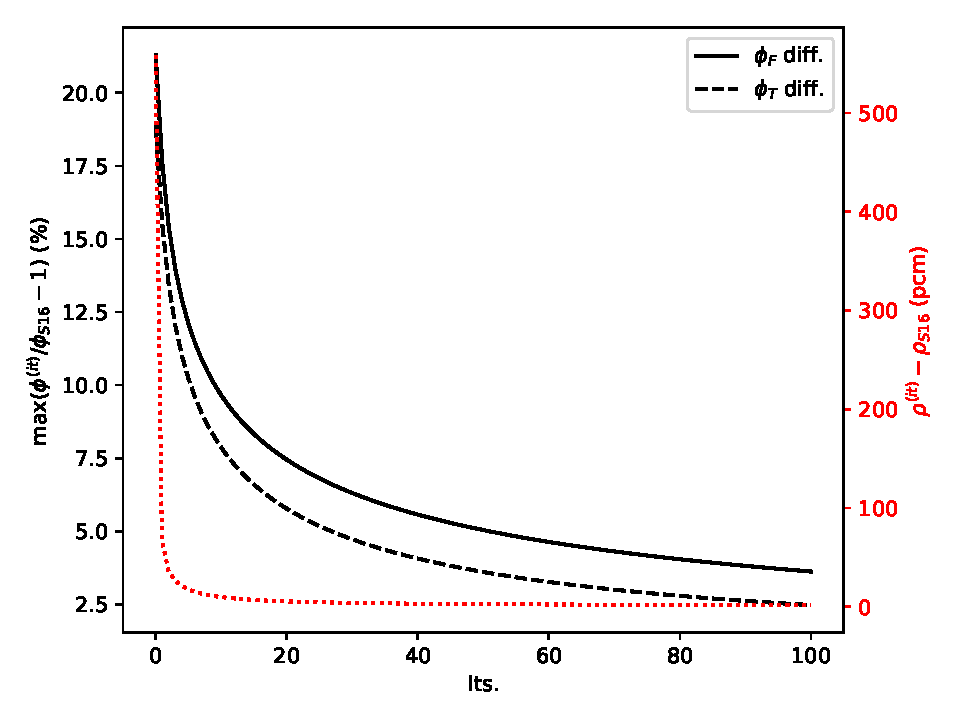
\includegraphics[width=.8\linewidth]{figures/kflxconv.pdf}
  \caption{Behavior of the convergence on the flux (right) and on the reacitivity (left) for $I = 200$.}
  \label{fig:kflx}
\end{figure}
%
\begin{figure}[hbtp]
  \centering
  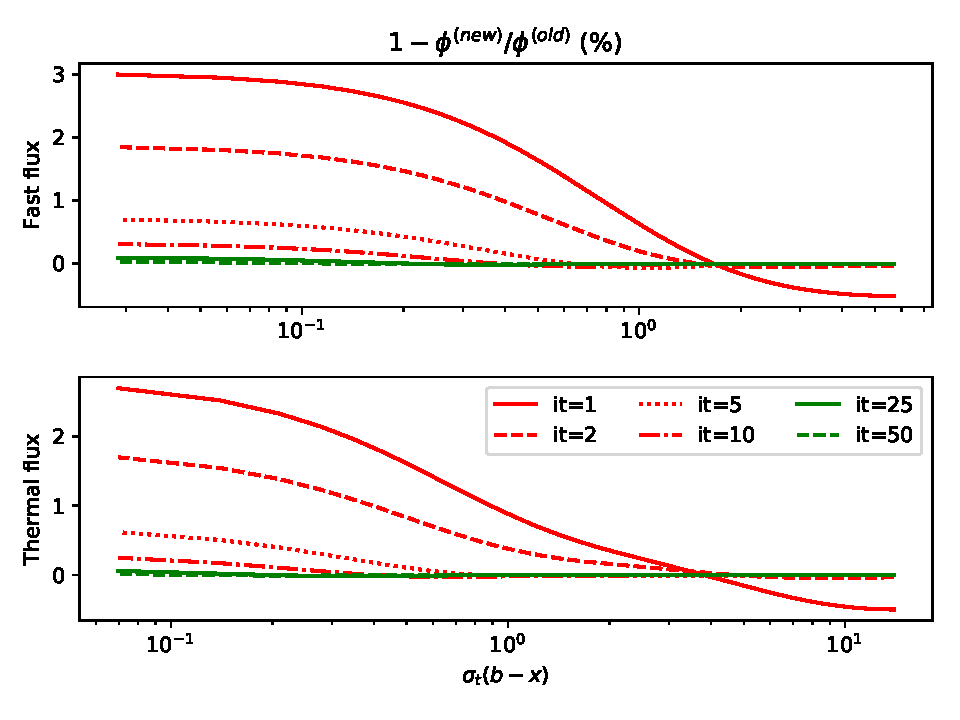
\includegraphics[width=.8\linewidth]{figures/eflxconv.pdf}
  \caption{Relative variation of the flux though the RM iterations ($I = 200$).}
  \label{fig:eflx}
\end{figure}

A one-group homogeneous problem is proposed hereafter in order to study the application of the Ronen method with angular redistribution in curvilinear geometries. Reference solutions are provided by collision probability method solvers, whose development take advantage of the implementation for the escape probabilities derived in section~\ref{sec:ce}. This choice is supported by the use of integral operators in the same Ronen method. Again, the implementation follows H\'ebert's textbook. The problems are solved in units of optical length, which means by simply setting the input total cross section equal to 1. The multiplying source becomes then $q = (c + \nu f) \phi_0 / 4\pi$, thus isotropic in angle, and with $c$ and $\nu f$ respectively as positive real numbers of secondaries per scattering and fission events. These numbers can be interpreted as conditional probabilities as well. The multiplicity $\nu$ acts as the eigenvalue of the problem. After the fundamental eigen-pair is known for given values of the constants and for a given size $L$, it is worthless to change $f$ alone to study the problem since only the product $\nu f$ counts for the balance (associated to the same eigenfunction). We choose then $f = 1$, ending up in only two free parameters for our study: $c_s$ and $L$. Even if this choice is unphysical for the assumed value of the total cross section together with $c > 0$, physical meaning is recovered by the fundamental value of $\nu$.

\textcolor{red}{Roy will be able to check these assertions in the coming days.}

\textcolor{blue}{The source assumes this form because the integration variables also have to the normalized by the mean free path (i.e. multiplied by the total cross section).}

\textcolor{green}{The use of the integral transport eqn. to get reference solutions is motivated by two main reasons. The first is to use again what we're implementing now for the escape probabilities. The second is to get the reference solution by inverting the operator used in the RM. So that we'll really know what is the solution to match. Furthermore, this won't be affected by ray effects of any kind. Lastly, we'll have to be very careful to the endpoint singularity when computing the collision probabilities.}

\section{CONCLUSION}
\label{sec:cncls}

The Ronen Method was firstly proposed for better estimates of the diffusion coefficient by calculating the current with a higher-order transport operator and a known best-estimate neutron flux. This originates an iterative scheme leading to new flux distributions solved by a diffusion solver yet with the aim to fulfill the integral transport equation. The direct resolution of the integral equation would imply the inversion of large matrices, with poor control of their conditioning. The solution of the diffusion equation offers many numerical advantages instead, solution speed and robustness above all.

Nonetheless, the same current can be enforced in the discretized form of the diffusion equation as suggested by the CMFD, which avoids the numerical issues arising with flat flux. This is the option adopted in this work. The implementation of the boundary conditions is improved to reproduce the expected vanishing current in case of reflection.

We obtain more accurate results for the two-group benchmark problem reported in \cite{tomatis2011application}. The final version of the article will show the results of the application of the method in the curvilinear coordinate systems, still using isotropic sources. In general, slow convergence is observed for the scalar flux, whose larger discrepancy with respect to the reference is always located on the vacuum boundary. Although the method is converging to the reference results provided by a discrete ordinate transport code, the improvement of the convergence rate and the use of coarser meshes are crucial for the advancement of the methodology in practical applications. These topics will be addressed as future developements.


\section*{ACKNOWLEDGMENTS}

The authors express their gratitude to Prof. Yigal Ronen who initiated the method.

\appendix
\section{APPENDIX. Gauss-quadratures}
\label{sec:apx_Flurig}

The integrals used in the calculation of the probabilities in the cylindrical and spherical frames are in the form:
\[
  I = \int_{r_{i-1/2}}^{r_{i+1/2}}{dh K(\ell(h))},
\]
and they are often evaluated numerically by Gauss-quadratures. The integrand can show an endpoint singularity in the first derivative when integrating in the convex regions, since $d_h K = \partial_{\ell} K\, \partial_{\ell}h$ and 
\[
  \lim_{h \rightarrow r_{i+1/2}}
    \frac{-2h}{\sqrt{r_{i+1/2}^2 - h^2}} = -\infty,
\]
for $\ell = 2\sqrt{r_{i+1/2}^2 - h^2}$ \cite{hebert2009applied}.
The use of a Gauss-Legendre quadrature with $N$ points in the integration interval is a good choice only if the integrand is continuous over the interval up to order $2N$. Gauss-Legendre quadrature integrates exactly polynomials of degree less than $2N$. The definite integrals can be regularized by a proper change of variable following the Flurig scheme, which yields a Gauss-Jacobi quadrature scheme \cite{carlvik1966integral}. We propose herafter a general change of variable to obtain both schemes at once:
\begin{equation}
\label{eq:varchange}
  \varrho = 1 - 2 \left(
      \frac{r_{i+1/2} - h}{\Delta r_i} \right)^{(1-\alpha/2)}
\end{equation}
with $\Delta r_i = r_{i+1/2} - r_{i-1/2}$ that yields
\begin{equation}
\label{eq:quad}
  I = \frac{\Delta r_i}{2}\int_{-1}^{1}{
    d\varrho (1-\varrho)^\alpha
%             (1+\varrho)^\beta
             K(\ell(\varrho))}
    = \sum_{n=1}^N{w_n K(\ell(h_n))},
\end{equation}
with the Gauss-Legendre scheme for $\alpha = 0$ and the Gauss-Jacobi scheme for $\alpha = 1$. %with the Gauss-Legendre scheme for $a=1$ ($\alpha = 0$, $\beta = 0$) and the Gauss-Jacobi scheme for $a=1/2$ ($\alpha = 1$, $\beta = 0$).
After retrieving the weights $v_n$ and the roots $\varrho_n$ of the selected $N$-point quadrature in $[-1, +1]$, the weights and roots to use in Eq. \ref{eq:quad} are respectively:
\begin{equation}
\label{eq:wnrn}
  w_n = \frac{\Delta r_i}{2} v_n \quad \text{and} \quad
  h_n = r_{i+1/2}
      - \left(\frac{1-\varrho_n}{2}\right)^{(1+\alpha)}
        \Delta r_i.        
\end{equation}
Weights and roots are obtained by the Scipy v1.4.1 library (special.roots\_jacobi) and Numpy v1.18.2 (polynomial.legendre.leggauss). We note that the values from these libraries are different from the ones printed in the cited textbooks \cite{hebert2009applied,stamm1983methods}.


\section{APPENDIX. Direct solution of integral transport by the collision probabilty method}
\label{sec:CPMsolution}

The integral transport equation for the scalar flux can be written using the first flight collision probabilities as \cite{hebert2009applied}:
\begin{subequations}
\label{eq:cmp_eqn}
\begin{equation}
\label{eq:cmp1_eqn}
V_i \sigma_i \phi_i = \sum_{j=1}^I {q_j V_j \tilde{p}_{ij}}
                    + J^{(-)}_{b}S_{b} \tilde{p}_{ib},
\end{equation}
where $b$ stands for any boundary with a non-zero entering current. $b=I+1/2$ for the cylindrical and for the spherical geometries, whereas two incoming currents can be present in the slab. This equation can be simplified further by using the reciprocity property from Eqs. \ref{eq:reciprocity},
\begin{equation}
\label{eq:cmp2_eqn}
\phi_i = \sum_{j=1}^I {q_j p_{ji}} + J^{(-)}_{b} \tilde{e}_{bi}
\end{equation}
\end{subequations}
with the reduced escape probability $p_{ji} = \tilde{p}_{ji} / \sigma_j$ and the escape probability counting for both the signed terms. The incoming current at the boundary can be given as fixed external source, or being expressed as proportional to the out-going current by means of the albedo $0 \leq \beta \leq 1$, like
\begin{equation}
\label{eq:albedo}
  J^- = \beta J^+ = \beta \left(
      \sum_{j=1}^I {q_j p_{jb}} + \tilde{t} J^-
    \right),
\end{equation}
with the reduced collision probability from the surface at $x_b$ thanks again to reciprocity. About \ref{eq:reciprocity2}, reciprocity considers entering neutrons distributed according to the cosine described by the direction of flight and the normal to the same surface, yielding a cosine current by $J^\pm = \phi/4$, suitable to reproduce white reflection with $\beta = 1$. %yields the white reflection, that is isotropic inwards redistribution of the outgoing current, regardless of the outgoing direction.
The transmission $\tilde{t}$ is the probability that a neutron enters the outer surface with the cosine distribution, travels  inwards and leaves it back again without colliding. Conservation implies that $\tilde{t} = 1 - \sum_j{\tilde{p}_{jb}}$.

The source term considers only isotropic emission, and it is composed by scattering and fission production as in Eq. \ref{eq:srclg0}. In absence of external sources, the problem becomes homogeneous with the multiplication factor $k$ assuming the role of eigenvalue to avoid the only vanishing solution. Eqs. \ref{eq:cmp_eqn} hold for any energy group, whose index is dropped for simplicity.

We setup hereafter an algebraic system equations for the unknown flux array $\vec{\phi}$ of size $(I \times G)$, flattened with the index of the spatial mesh running first. The extension of the solution method to problems with external sources in submultiplicative media is straightforward. Eq. \ref{eq:cmp2_eqn} for bare bodies, that is in presence of vacuum boundary condition, is rewritten as:
\begin{equation}
\label{eq:cpm_syseqns}
(\mathbf{I} - \mathbf{P}\mathbf{S}) \vec{\phi}^{(n+1)} = \mathbf{P} (\chi \otimes \mathbf{F}) \vec{\phi}^{(n)} / k^{(n)},
\end{equation}
where the index $n$ addresses power method iterations to solve the eigenvalue problem. All matrices in Eq. \ref{eq:cpm_syseqns} are constructed by blocks. The matrix $\mathbf{P}$ is block diagonal with all (transposed) matrices of reduced collision probabilities per group, placed in increasing order from the fast groups, which are assigned to the lowest values of the index $g$ as usual. The matrix $\mathbf{S}$ is composed by $G \times G$ diagonal blocks with elements $[\sigma_{s, g \leftarrow g',j}\delta_{ij}, \, i, j=1, \ldots, I]$, contrary to the matrix $\mathbf{F}$ which has only G blocks set by columns and with elements $[\nu\sigma_{f, g, j}\delta_{ij}, \, i, j=1, \ldots, I]$. The new estimate of the flux vector is computed by multiplying the left side of the equation by the inverse of the removal matrix, i.e. $(\mathbf{I} - \mathbf{S} \mathbf{P})^{-1}$, assuming that it is invertible. The new estimate of the eigenvalue can be obtained by enforcing neutron conservation through the iterations, while achieving the convergence:
\[
  k^{(n+1)} = k^{(n)}
    \frac{\langle \vec{\phi}^{(n+1)} | \mathbf{F} \vec{\phi}^{(n+1)} \rangle}{\langle \vec{\phi}^{(n+1)} | \mathbf{F} \vec{\phi}^{(n)} \rangle}.
\]
The full eigen-spectrum can be obtained by resolving the problem for the fission production reaction rates, showing smaller rank. First, note that $(\chi \otimes \mathbf{F}) = \mathbf{X} \mathbf{F}$, with $\mathbf{X}$ built by $G$ diagonal blocks stacked per row of the form $[\chi_{g,j}\delta_{ij}, \, i, j=1, \ldots, I]$. The eigen-solver operates then on the matrix $\mathbf{F}(\mathbf{I} - \mathbf{S} \mathbf{P})^{-1} \mathbf{P} \mathbf{X}$.

In case of partial currents given by an albedo relation at the boundary, the same solving scheme still holds after redefinition of the matrix $\mathbf{P}$:
\[
\mathbf{P} \leftarrow \mathbf{P} + \frac{\beta}{1 - \beta \tilde{t}} \mathbf{E},
\]
with $\mathbf{E}=[\tilde{e}_{bi} p_{jb},\; 1 \leq i,j \leq I]$.

\setlength{\baselineskip}{12pt}
% warning: the style plain may not be the one of the conference
\bibliographystyle{unsrt}
\bibliography{RonenMethod}

\end{document}
